% Chapter Template

\chapter{Quantum Dots} % Main chapter title

\label{sec:Quantum_Dots} % Change X to a consecutive number; for referencing this chapter elsewhere, use \ref{ChapterX}

%----------------------------------------------------------------------------------------
%	SECTION 1
%----------------------------------------------------------------------------------------

\section{Fundaments}

A quantum dot (QD) existentially a small ``box'' filled with particles. When the size of this region is comparable to the wavelength of the particle that populates it, the system becomes quasi 0-dimensional, exhibiting a discrete energy spectrum. This is somehow similar to an atoms, and this is why QD's are usually called artificial atoms. The dots can be filled with electrons or holes, depending on which atoms the substrate is doped with. Different sites can be coupled via tunnel barriers, allowing the particles to ``jump'' from one dot to another. It is also common to couple a source and a drain reservoir that enable the exchange of particles. By attaching current and voltage probes to these reservoirs we can measure the electronic properties of the device. This description of a QD is very general, and this is why exist systems of may different sizes and materials. For instance self-assembled quantum dots, semiconductor lateral and vertical dots, or even carbon nanotubes. An example of this devices can be found in Fig.~\ref{fig:different_devices}. In this work, we focus on lateral gated semiconductor quantum dots. These devices allow a great control over the different parameters of the system, what can be used to tune it's values in situ. 
\begin{figure}[!htbp]
	\centering
	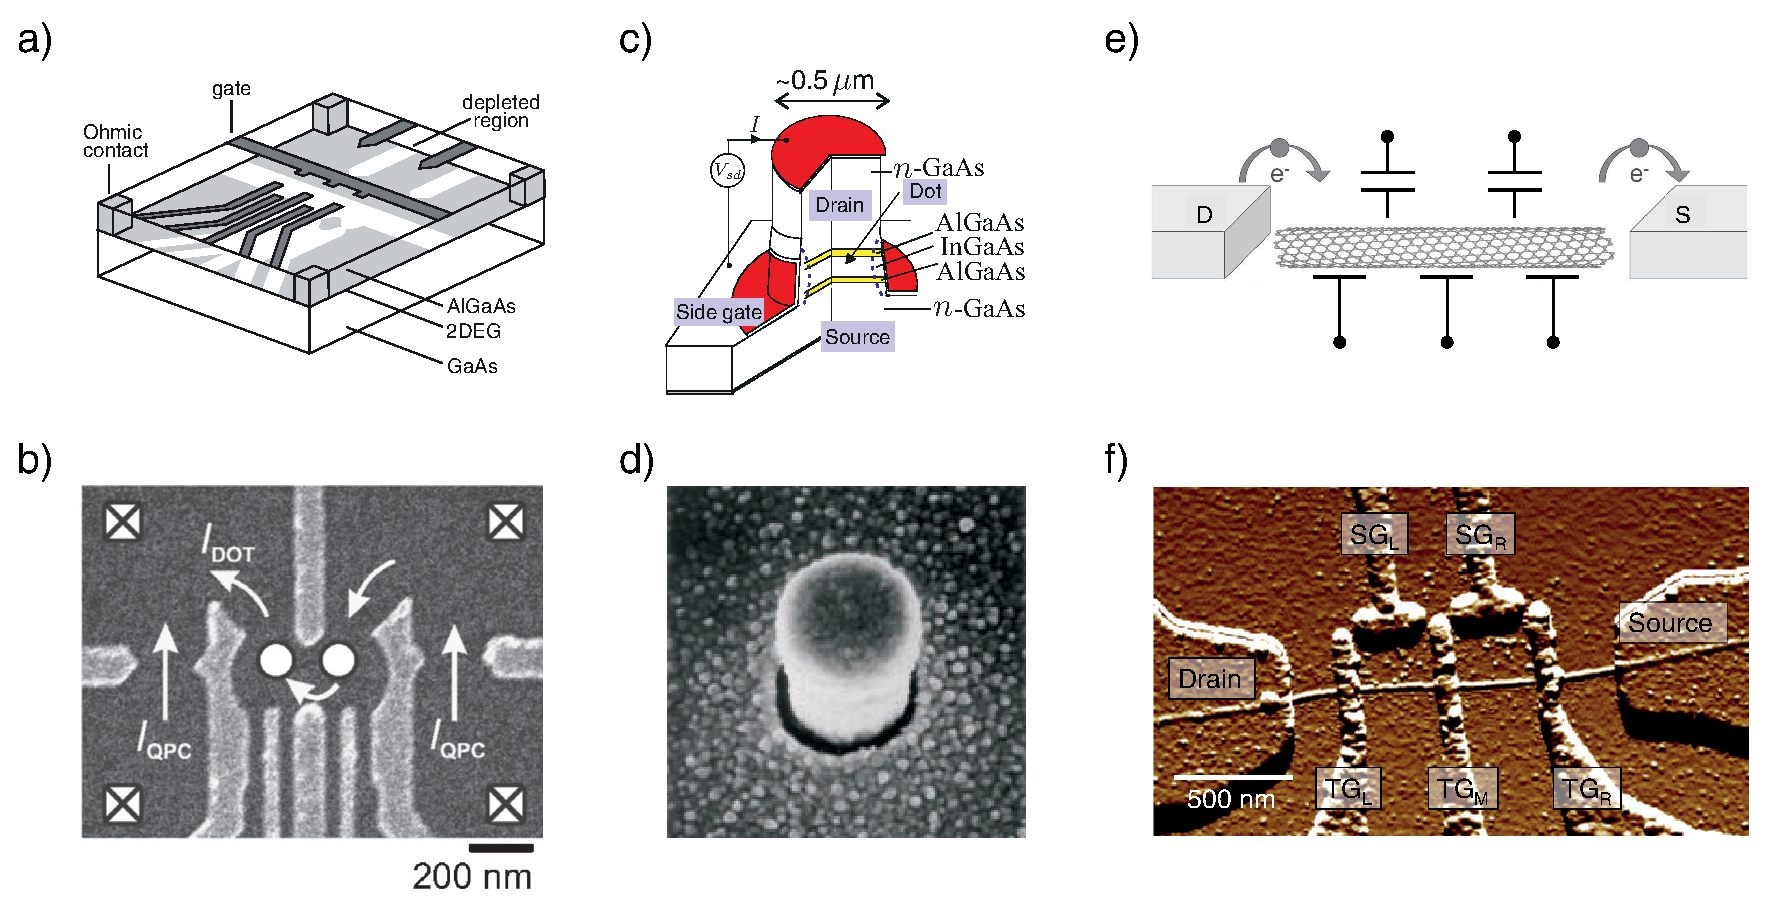
\includegraphics[width=\linewidth]{different_devices.eps}
	\caption{Different devices for quantum dots. a) Schematic view and b) scanning electron micrograph (SEM) of a lateral DQD, taken from ref. \cite{Hanson2007}. c) Schematic and d) SEM images of a vertical semiconducting QD, taken from ref. \cite{Kouwenhoven2001}. e) Schematic and f) atomic force microscope (AFM) of a DQD implemented in a carbon nanotube, taken from e) ref. \cite{SapmazPhd} and f) ref. \cite{Sapmaz2006}.}
	\label{fig:different_devices}
\end{figure}

Fabrication of gated quantum dots starts with a layered heterostructure composed by different semiconducting materials. A common choice for the semiconductors is GaAs and AlGaAs grown on top of each other. By doping the n-AlGaAs with Si we can introduce free electrons, which are accumulated in the interface forming a 2-dimensional electron gas (2DEG)\cite{Elzerman2005}. If we are interested in holes instead of electrons we can keep the GaAs/AlGaAs heterostructure undoped\cite{Tracy2014}. By applying negative voltages to metal surface electrodes (gates) on top of the semiconductor heterostructure the 2DEG is locally depleted, thereby forming the QD. In order to control the electrostatic potential of the dots with respect to the reservoirs we can couple it capacitively to a gate electrodes. The tunneling rate can be also modified with electric fields applied to the gates located between neighbouring dots. With this we have an all-electrical control over the system. We can also use a magnetic field to produce a Zeeman splitting in the spin of the particles.

\section{Transport}
The charge transport thought the system is a perfect way to measure the state of the device, since the intensity observed depends on the states of the particles inside the quantum dots. in the contacts (source and drain) there are free particles with energies up to the chemical potential $\mu$. At low temperatures this chemical potential corresponds to the Fermi energy. During the entire chapter we will consider that the temperature of the device is low enough so the approximation of the chemical potential as a step function is justified. Applying a voltage difference between the two reservoirs known as the bias voltage $V_{\text{bias}}$. The relation between this three parameters is
\begin{equation}
	V_{\text{bias}}=\frac{\mu_R-\mu_L}{e}\; ,
\end{equation}
where $L$ and $R$ denote the left and right contact respectively, and $e$ is the electron charge. The choice of the sign is a convention, different choices can be found in the literature. The chemical potential for the quantum dots is defined as the required energy to add a new particle in the site. The more particles there are in the QD, the higher is the chemical potential, thus forming what is known as the electrochemical ladder. All this discrete levels can be shifted by the gate voltage $V_G$. This is depicted in Fig.(\ref{fig:potential_ladder}). If the chemical potential of a reservoir ir larger than $\mu(N)$, then one particle can enter in the quantum dot. This will occur until the QD's potential reaches a value higher than the contact $\mu(N+1)>\mu_i$. The same thing will happen in reserve, if $\mu(N)>\mu_i$, the particles will leave the system towards the reservoir until a balance is reached. In the example shown two particles can enter initially in the QD from the right reservoir, but only one of then can tunnel out to the left drain. Then a net intensity of one particle will flow continuously from right to left.
\begin{figure}[!htbp]
	\centering
	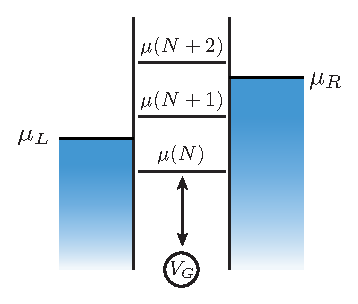
\includegraphics[width=0.4\linewidth]{potential_ladder.eps}
	\caption{Sketch of the electrochemical ladder in a quantum dot. The energy origin is given by the gate voltage $V_G$.}
	\label{fig:potential_ladder}
\end{figure}

In order to know exactly the number of particles inside the devices we must use the stability diagrams. This kind of measures can be obtained by two different techniques, but with very similar results. In both of them the chemical potential of the reservoirs are keep constant and equal to each other, that is $V_{\text{bias}}=0$. Then the gate voltages of each dot are modified independently, trying to map out as much of the area as possible. The aim of these measures is to obtain at which values fir the gate voltages there is a variation in the number of particles. One possibility for this is the use of a quantum point contact (QPC), which is sensitive to the variation of charge inside the QD. On the other hand, we can determine this movement of the particles also via the charge intensity. Both methods assume a sequential tunneling, that is, only one particle enter or exit the device at each time, so every time a transition is measured, either with the QCP or with the electronic intensity, we can assure that only one particle has changed its position. Once we don't see any more transitions all the QD's are empty, allowing us to define the exact number of particles for each quantum dot in each region.

\subsection{Coulomb Blockade}

\subsection{Pauli Blockade}

\section{Quantum Gates with QD}

